\subsection{The Boot Process}
\label{sec:booting}

When a computer is powered up, it undergoes a \textit{bootstrapping} process,
also called \textit{booting}, for simplicity. Although many steps in the boot
process depend on the motherboard and components in a computer, the process
does follow a high-level structure that is prescribed in the SDM. This section
provides the details needed to analyze SGX's security properties.
\cite{intel2010booting} provides a good reference on the entire booting
process.

\subsubsection{UEFI Platform Initialiaztion}
\label{sec:efi}

The firmware in modern computers using the Intel architecture implements the
\textit{Platform Initialization} (PI) process in the \textit{Unified
Extensible Firmware Interface} (UEFI) specification \cite{forum2015uefi}. The
platform initialization follows the steps shown in Figure~\ref{fig:uefi} and
described below.

\begin{figure}[hbt]
  \center{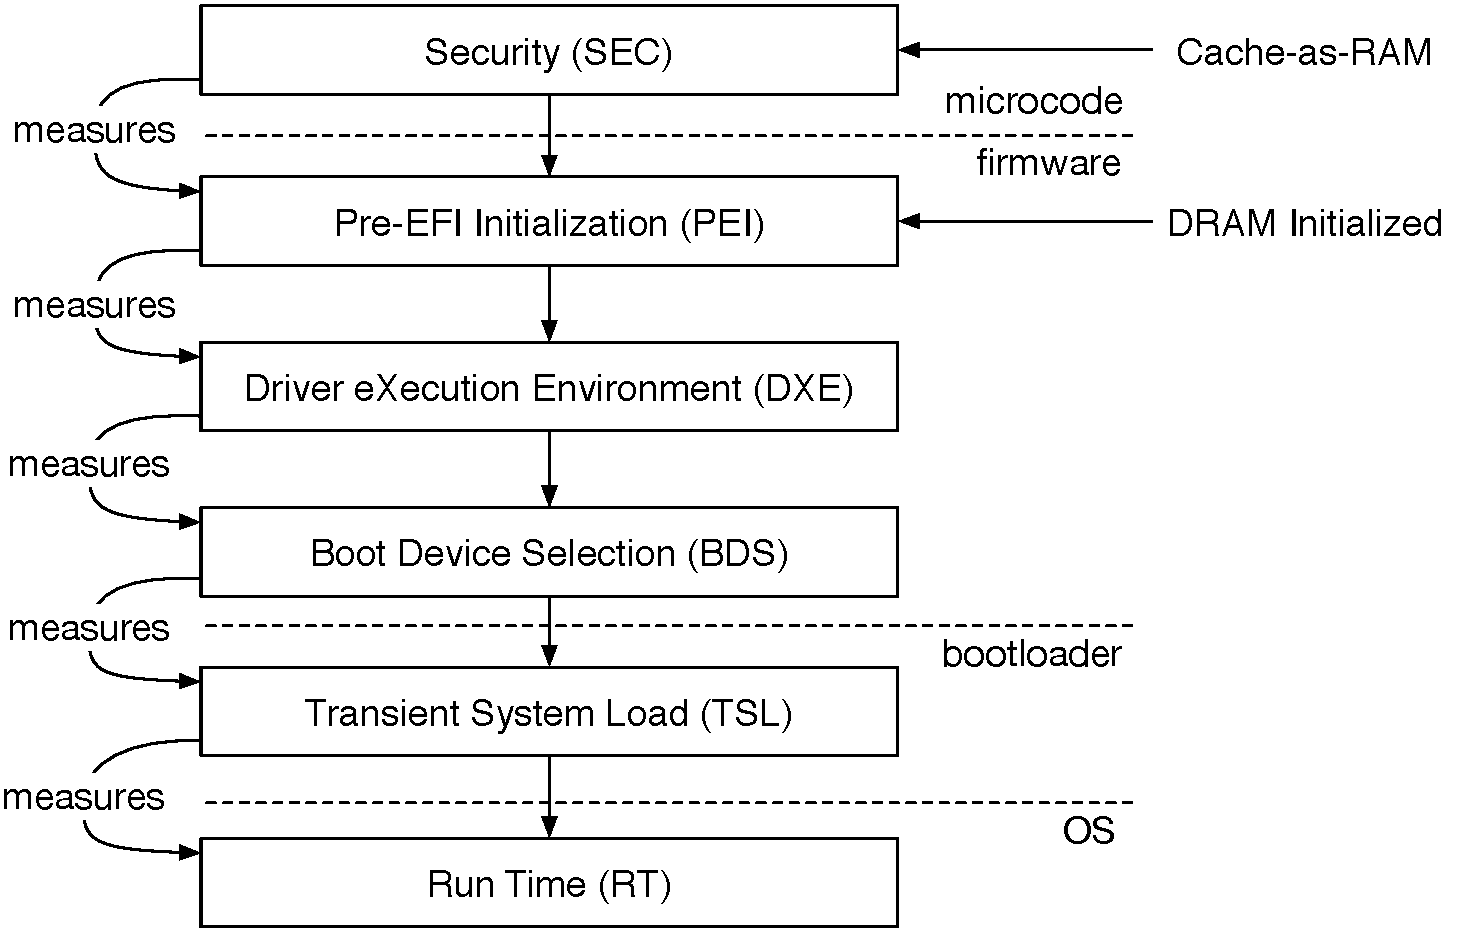
\includegraphics[width=75mm]{figures/uefi.pdf}}
  \caption{
    The stops on the ring interconnect used for inter-core and core-uncore
    communication.
  }
  \label{fig:cpu_uncore}
\end{figure}

The computer powers up, reboots, or resumes from sleep in the
\textit{Security phase} (SEC). The SEC implementation is responsible for
establishing a temporary memory store and loading the next stage of the
firmware into it. The SEC implementation also performs any security-related
tasks, such as measuring (computing a cryptographic hash of) the next firmware
stage, and potentially aborting if the firmware is not signed by a pre-approved
key.

SEC is followed by the \textit{Pre-EFI Initialization phase} (PEI), which
initializes the computer's DRAM, copies itself from the temporary memory
store into DRAM, and tears down the temporary storage. When the computer is
powering up or rebooting, the PEI implementation is also responsible for
initializing all the non-volatile storage units that contain UEFI firmware and
loading the next stage of the firmware into DRAM. When recovering from sleep

PEI hands off control to the \textit{Driver eXecution Environment phase} (DXE).
In DXE, a loader locates and starts firmware drivers for the various components
in the computer. DXE is followed by a Boot Device Selection (BDS) phase, which
is followed by a Transient System Load (TSL) phase, where an EFI application
loads the operating system selected in BDS. Last, the OS loader passes control
to the operating system's kernel, entering the Run Time (RT) phase.

On a system that uses secure boot or attestation, the SEC implementation is the
system's root of trust. Each platform initialization phase is responsible for
verifying or measuring the firmware that implements next phase. For example, in
a TPM / TXT system, SEC firmware initializes the TPM registers that hold the
system's measurement, which are the Platform Configuration Registers (PCRs) for
the Static Root of Trust Measurement (SRTM). The SEC implementation then stores
the PEI's measurement (cryptographic hash) into a measurement register. In
turn, the PEI implementation measures the DXE firmware and updates the
measurement register that stores the PEI hash to account for the DXE hash. When
the OS is booted, the hash in measurement register accounts for all the
firmware that was used to boot the computer.


\subsubsection{CPU Hardware Initialization}
\label{sec:cpu_init}

% Initialization Overview: SDM S 9.1

Right after a computer is powered up, all the logical processors (LPs) on the
motherboard undergo \textit{hardware initialization}, which invalidates the
caches (\S~\ref{sec:caching}) and TLBs (\S~\ref{sec:tlbs}), performs a
\textit{Built-In Self Test} (BIST), and sets all the registers
(\S~\ref{sec:registers}) to pre-specified values.

% Multiple-Processor Initialization: SDM S 8.4
% BSP and AP Processors: SDM S 8.4.1
% MP Initialization Protocol Algorithms for MP Systems: SDM S 8.4.3
% An ivy bridge CPUID: family 06h, extended model 3, model 58, stepping 9

After hardware initialization, the LPs perform the Multi-Processor (MP)
initialization algorithm, which results in one LP being selected as the
\textit{bootstrap processor} (BSP), and all the other LPs being classified as
\textit{application processors} (APs).

According to the SDM, the details of the MP initialization algorithm for recent
CPUs depend on the motherboard and firmware. In principle, after completing
hardware initialization, all LPs attempt to issue a special no-op transaction
on the QPI bus. A single LP will succeed in issuing the no-op, thanks to
the QPI arbitration mechanism, and to the UBox (\S~\ref{sec:cache_coherence})
in each CPU package, which also serves as a ring arbiter. The arbitration
priority of each LP is based on its APIC ID (\S~\ref{sec:interrupts}), which is
provided by the motherboard when the system powers up. The LP that issues the
no-op becomes the BSP. Upon failing to issue the no-op, the other LPs become
APs, and enter the \textit{wait-for-SIPI} state.

% Typical BSP Initialization Sequence: SDM S 8.4.4.1

The SDM describes a legacy boot sequence, where BSP sets its RIP register to
0xFFFFFFF0 (16 bytes below 4GB), where the firmware is expected to place a
instruction that jumps into the PEI implementation. This is unfortunate, as
recent processors dropped support for this approach
\cite{reinauer2013fitpatch}.

Modern firmware implementations instead contain a Firmware Interface Table
(FIT), which was introduced by an Intel patent \cite{qureshi2006fit} in the
context of Intel's Itanium architecture. The FIT use in Intel's current 64-bit
architecture is described in a patent \cite{datta2013acm} and briefly
documented in a TXT lab note \cite{intel2010txtlab}.

The use of TXT requires firmware that contains a FIT and Intel-supplied ACMs
\cite[p. 92]{futral2013servertxt}.


BIOS
The BSP sets its RIP register to point to the firmware reset code, which must
be present at 0xFFFFFFF0 (16 bytes below the 4 GB mark). This is accomplished
by having the initial SAD (\S~\ref{sec:cache_coherence}) and PCH
(\S~\ref{sec:motherboard}) configurations map the 4 KB below the 4 GB mark of
the memory address space (\S~\ref{sec:address_spaces}) to the SPI flash chip
that stores the motherboard's firmware.

\subsubsection{Boot Firmware}
\label{sec:firmware_boot}

\cite{intel2010booting} and \cite{coreboot2015manual} describe the
initialization steps performed by the firmware, from an implementor's
perspective. A few steps are interesting from the perspective of SGX and
caching attacks.

% Preventing Caching: SDM S 11.5.3

When the BSP starts executing firmware code, DRAM is not available. The
firmware places the BSP in \textit{Cache-as-RAM} (CAR) mode to be able to use a
call stack and other high-level constructs. Ater CAR is enabled, the memory
initialization code, which is typically Intel's \textit{Memory Reference Code}
(MRC), is loaded into the cache. When executed, the memory initialization code
discovers the DRAM chips connected to the motherboard and sets them up, and
enables and configures the memory controllers.

After DRAM becomes available, the boot firmware is copied into DRAM and the BSP
is taken out of CAR mode. The BSP's LAPIC is initialized and used to send a
broadcast \textit{Startup Inter-Processor Interrupt} (SIPI) to wake up the
APs. The interrupt vector in a SIPI indicates the DRAM address of the firmware
code for initializing APs.

% Typical AP Initialization Sequence: SDM S 8.4.4.2


